%%%%%%%%%%%%%%%%%%%%%%%%%%%%%%%%%%%%%%%%%%%%%%%%%%%%%%%%%%%%%%%%%%%%%%%%%%%%%%%%%%%%%%%%%%%%%%%%%%%%%%%
\section{Hierarchical Ideal Point Topic Model}
\label{sec:c6_model}
%%%%%%%%%%%%%%%%%%%%%%%%%%%%%%%%%%%%%%%%%%%%%%%%%%%%%%%%%%%%%%%%%%%%%%%%%%%%%%%%%%%%%%%%%%%%%%%%%%%%%%%

Bringing topic models~\cite{blei-09} into ideal-point modeling
provides an interpretable, text-based foundation for political
scientists to understand why the models make the predictions they
do. However, both the \emph{topic}---what is discussed---and the
\emph{framing}---how it is discussed---also reveal political
preferences. We therefore introduce \emph{frame-specific} ideal
points, using a hierarchy of topics to model issues and their
issue-specific frames. Although the definition of ``frame'' is itself
a moving target in political science~\cite{Entman:JC93}, we adopt the
theoretically motivated but pragmatic approach of
\newcite{Nguyen:NIPS13}: just as agenda-issues map naturally to topics
in probabilistic topic models (e.g., \newcite{Grimmer:PA10}), the
frames as second-level agenda-setting \cite{McCombs:JS05} map to
second-level topics in a hierarchical topic model.

Our model's inputs are votes $\{v \subtwo ab\}$, each the response of
legislator $a \in [1,A]$ to bill $b \in [1,B]$. Two types of text
supplement the votes: floor speeches (documents) $\{\bm w_d\}$ from
legislator $a_d$, and the text $\bm w'_b$ of bill $b$.  While
congressional debates are typically about one piece of legislation,
we make no assumptions about the mapping between $\bm w_d$ and $\bm
w'_b$. In principle this allows $\bm w_d$ to be \emph{any} text by
legislator $a_d$ (e.g., not just floor speeches about this bill, but
blogs, social media, press releases) and---unlike Gerrish and
Blei~\shortcite{Gerrish:ICML11}---this permits us to make predictions
about individuals even without vote data for
them. Figure~\ref{fig:c6_hiptm} shows the plate notation diagram of
\name{}, which has the following generative process:

\begin{small}
\begin{enumerate*}
  \item For each issue $k \in [1,K]$
  \begin{enumerate*}
    \item Draw $k$'s associated topic $\phi_k \sim~\Dir {\beta, \phi_k^{\star}}$
    \item Draw issue-specific distribution over frames $\psi_k \sim \GEM {\lambda_0}$
    \item For each frame $j \in [1, \infty)$ (specific to issue $k$)
    \begin{enumerate*}
      \item Draw $j$'s associated topic $\phi \subtwo kj \sim \Dir {\beta, \phi_k}$
      \item Draw $j$'s regression weight $\eta \subtwo kj \sim \mathcal{N}(0, \gamma)$
    \end{enumerate*}
  \end{enumerate*}
  \item For each document $d \in [1,D]$ by legislator $a_d$
  \begin{enumerate*}
    \item Draw topic (i.e., issue) distribution $\theta_d \sim~\Dir \alpha$
    \item For each issue $k \in [1,K]$, draw frame distribution $\psi \subtwo dk \sim \DP \lambda {\psi_k}$
    \item For each token $n \in [1, N_d]$
    \begin{enumerate*}
      \item Draw an issue $z \subtwo dn \sim~\Mult {\theta_d}$
      \item Draw a frame $t \subtwo dn \sim \Mult {\psi \subtwo d {z \subtwo
          dn}}$
      \item Draw word $w \subtwo dn \sim~\Mult {\phi \subtwo {z \subtwo dn}{t \subtwo
          dn}}$
    \end{enumerate*}
  \end{enumerate*}
  \item For each legislator $a \in [1, A]$ on each issue $k \in [1, K]$
  \begin{enumerate*}
    \item Draw issue-specific ideal point
    $u \subtwo ak \sim \mathcal{N}(\sum_{j=1}^{J_k} \hat{\psi} \subthree akj \eta \subtwo kj, \rho)$
      weighting $\eta \subtwo kj$ by how much the legislator talks about that frame
  \end{enumerate*}
  \item For each bill $b \in [1, B]$
  \begin{enumerate*}
    \item Draw polarity $x_b \sim \mathcal{N}(0, \sigma)$
    \item Draw popularity $y_b \sim~\mathcal{N}(0, \sigma)$
    \item Draw topic (i.e., issue) proportions $\vartheta_b \sim \Dir \alpha$
    \item For each token $m \in [1, M_b]$ in the text of bill $b$
    \begin{enumerate*}
      \item Draw an issue $z' \subtwo bm \sim~\Mult {\vartheta_b}$
      \item Draw a word type $w' \subtwo bm \sim~\Mult {\phi_{z' \subtwo bm}}$
    \end{enumerate*}
  \end{enumerate*}
  \item For each vote $v \subtwo ab$ of legislator $a$ on bill $b$
  \begin{enumerate*}
    \item $p(v \subtwo ab \given \bm u_a, x_b, y_b,\hat{\vartheta}_b) =~\Phi\left(x_b \sum_{k} \hat{\vartheta} \subtwo bk u \subtwo ak + y_b\right)$
  \end{enumerate*}
\end{enumerate*}
\end{small}

\begin{figure}[t]
\centering
  \includegraphics[width=.8\linewidth]{\figfile{hiptm}}
  \caption{Plate notation diagram of \name{}.}
  \label{fig:c6_hiptm}
\end{figure}

\paragraph{Topic Hierarchy.} With the goal of analyzing agendas and
frames in mind, our topic hierarchy has two levels: (1) \textit{issue
  nodes} and (2) \textit{frame nodes}.
(Look ahead to Figure~\ref{fig:frames} for an illustration.)
More specifically, there are
$K$ issue nodes, each with a topic $\phi_k$ drawn from a Dirichlet
distribution with concentration parameter $\beta$ and a prior mean
vector $\phi_k^{\star}$, i.e., $\phi_k \sim \Dir {\beta,
  \phi_k^{\star}}$.  In this hierarchical structure, first-level nodes
map to agenda issues, which we treat as non-polarized, and
second-level nodes map to issue-specific frames, which we assume
polarize on the issue-specific
dimension.\footnote{\newcite{Nguyen:NIPS13} allow first-level nodes to
  polarize but find first-level nodes are typically neutral.}

\begin{table}[t!]
\centering \small
\begin{tabular}{p{.95\linewidth}}
  \hline
  \textbf{{Agriculture}}:
    food; agriculture; loan; farm; crop; dairy; rural; conserve; commodity; eligible; farmer; margin; milk; contract; nutrition; livestock; plant \\ \hline
\ignore{
  \textbf{{Banking, Finance, and Domestic Commerce}}:
    insure; bank; patent; mortgage; loan; commission; issuer; director; fee; application; contract; transaction; property; internet; flood\_insurance; code; file\\ \hline
  \textbf{{Defense}}:
    unit; army\_force; transfer; army; contract; acquisition; subsection; air\_force; homeland\_security; nuclear; personnel; public\_law; nation\_defense; navy; command \\ \hline
  \textbf{{Energy}}:
    oil; electricity; fuel; shelf; outer\_continent; pipeline; facility; environment; qualification; renew\_energy; energy\_efficiency; interior; energy\_policy; exploration \\ \hline}
  \textbf{{Health}}:
    drug; medicine; coverage; disease; public\_health; hospital; social\_security; health\_insurrance; patient; application; treatment; payment; physician; nurse; clinic\\ \hline
  \textbf{{Labor, Employment, and Immigration}}:
    employment; immigration; labor; paragraph; eligible; status; compensation; application; wage; homeland\_security; unemployment; board; violation; file; perform; mine \\ \hline
\ignore{  \textbf{{Social Welfare}}:
    social\_security; disable; eligible; payment; social; food; nutrition; insurance; employment; income; poverty; earn;  calendar \\ \hline
  \textbf{{Transportation}}:
    transport; highway; motor\_vehicle; metropolitan; airport; freight; rail; carrier; chapter; driver; motor; october; traffic; paragraph; surface\_transport \\ \hline}
\end{tabular}
\caption{Examples of informed priors $\phi_k^{\star}$ for issues.}
\label{tab:c6_prior}
\end{table}

To improve topic interpretability, issue nodes have an informed prior
from the Congressional Bills Project $\{\phi_k^{\star}\}$
(Table~\ref{tab:c6_prior}).\footnote{The Congressional Bills Project
  provides a large collection of labeled congressional bill text.  We
  compute $\{\phi_k^{\star}\}$ as the empirical word distribution from
  all bills labeled with $k$. $K=19$, corresponding to 19 major topic
  headings in the Policy Agendas Project Topic Codebook. } The frame
topic $\phi \subtwo kj$ at each frame node is a Dirichlet draw
centered at the corresponding (parent) issue node. While the number of
issues is fixed \textit{a priori}, the number of second-level frames
is unbounded.  We also associate each second-level frame node with an
ideal point $\eta \subtwo kj \sim \mathcal{N}(0, \gamma)$. This
resembles how supervised topic
models~\cite{Blei:NIPS07:slda,Nguyen:NAACL15:anchor}
discover polarized topics' associated response variables.

\paragraph{Generating Text from Legislators.}
One of our model's goal is to study how legislators \textit{frame} policy agenda issues. To achieve that, we analyze congressional speeches (documents) $\{\bm w_d\}$, each of which is delivered by a legislator $a_d$. To generate each token $w \subtwo dn$ of a speech $d$, legislator $a_d$ will (1) first choose an issue $z \subtwo dn \in [1,K]$ from a document-specific multinomial $\theta_d$, then (2) choose a frame $t \subtwo dn$ from the set of infinitely many possible frames of the given issue $z \subtwo dn$ using the frame proportion $\psi \subtwo dk$ drawn from a Dirichlet process, and finally (3) choose a word type from the chosen frame's topic $\phi \subtwo {z \subtwo dn}{t \subtwo dn}$. In other words, our model generates speeches using a mixture of $K$ \hdp{}s ~\cite{Teh:JASA06:hdp}.\footnote{If we abandoned the labeled data from the Congressional Bills Project to obtain the prior means $\phi_k^{\star}$, it would be relatively straightforward to extend to a fully nonparametric model with unbounded $K$~\cite{Ahmed:ICML13:ncrf,Paisley:TPAMI14:nhdp}.}

\ignore{
One of our model's goals is to study how legislators \textit{frame}
policy agenda issues. To achieve that, we analyze congressional
speeches (documents) $\{\bm w_d\}$ from legislator $a_d$.  Our model
generates text in the speeches using a mixture of $K$
\hdp{}s~\cite{Teh:JASA06:hdp}.\footnote{If we abandoned the labeled
  data from the Congressional Bills Project to obtain the prior means
  $\phi_k^{\star}$, it would be relatively straightforward to extend
  to a fully nonparametric model with unbounded
  $K$~\cite{Ahmed:ICML13:ncrf}.}
}

\jbgcomment{There's a missing connection here.  How does it improve
  the model?}

\paragraph{Generating Bill Text.}
\label{subsec:c6_bill_text}
The bill text provides information about the policy agenda issues that each bill
addresses. We use \lda{} to model the bill text $\{\bm w'_b\}$. Each bill $b$ is
a mixture $\vartheta_b$ over $K$ issues, which is drawn from a symmetric
Dirichlet prior, i.e., $\vartheta_b \sim \Dir \alpha$. Each token $w' \subtwo
bm$ in bill $b$ is generated by first choosing a topic $z' \subtwo bm \sim \Mult
{\vartheta_b}$, and then choosing a word type $w' \subtwo bm \sim \Mult
{\phi_{z' \subtwo bm}}$, as in \lda{}.

\paragraph{Generating Roll Call Votes.}
\label{subsec:c6_vote}
Following recent work on multi-dimensional ideal
points~\cite{Lauderdale:AJPS14,Sim:AAAI15:utility}, we define the probability of
legislator $a$ voting ``Yes'' on bill $b$ as $p(v \subtwo ab = \mbox{Yes} \given
\bm u_a, x_b, y_b,\hat{\vartheta}_b) =$
\begin{equation}
\Phi\left(x_b \sum_{k=1}^K \hat{\vartheta} \subtwo bk u \subtwo ak + y_b\right)
\end{equation}
where $\hat{\vartheta}_b$ is the empirical distribution of bill $b$ over the $K$ issues and is
defined as $\hat{\vartheta} \subtwo bk = \frac{M \subtwo bk}{M \subtwo b{\cdot}}$. Here, $M \subtwo
bk$ is the number of times in which tokens in $b$ are assigned to issue $k$ and $M \subtwo
b{\cdot}$ is the marginal count, i.e., the number of tokens in bill $b$.

The ideal point of legislator $a$ specifically on issue $k$ is $u \subtwo ak$
and comes from a normal distribution
\begin{equation}
 \mathcal{N}(\hat{\psi} \subtwo ak^T \bm \eta_k, \rho) \equiv \mathcal{N}\left(\sum_{j=1}^{J_k} \hat{\psi} \subthree akj \eta \subtwo kj, \rho\right)
  \label{eqn:c6_idealpoint}
\end{equation}
where $J_k$ is the number of frames for topic $k$, which is unbounded. The mean
of the Normal distribution is a linear combination of the ideal points $\{\eta
\subtwo kj\}$ of all issue $k$'s frames, weighted by how much time legislator
$a$ spends on each frame when talking about issue $k$, i.e., $\psi \subthree akj
= \frac{N \subthree akj}{N \subthree ak{\cdot}}$. Here, $N \subthree akj$ is the
number of tokens authored by $a$ that are assigned to frame $j$ of issue $k$,
and $N \subthree ak{\cdot}$ is the marginal count. When $N \subthree ak{\cdot} =
0$, which means that legislator $a$ does not talk about issue $k$, we back off
to an uninformed zero mean.

\jbgcomment{``regress on'' should be more explicit}

Equation~\ref{eqn:c6_idealpoint} resembles how supervised topic models (\slda{}) link topics with a response, in that the response---the issue-specific ideal point $u \subtwo ak$---is latent. It is similar to how \newcite{Gerrish:ICML11} use the bill text to regress on the bill's latent polarity $x_b$ and popularity $y_b$. In this paper, we only use text from congressional speeches for regression, as these can capture how legislators frame specific topics. Incorporating the bill text into the regression is an interesting direction for future work.

\ignore{Equation~\ref{eqn:c6_idealpoint} resembles how supervised topic models (\slda{})
link topics with a response, in that the response, the issue-specific ideal
points $u \subtwo ak$, is latent. Like \newcite{Gerrish:ICML11}, we use the bill
text to regress on the bill's latent polarity $x_b$ and popularity $y_b$. We
only use text from congressional speeches for regression, as these can capture
how legislators frame specific topics. Incorporating the bill text into the
regression is an interesting direction for future work.
}

%\section{Ideal Point Models}
%\label{sec:ideal_point} Ideal point models are methods to estimate the position of voters and bills
%given the observable votes. More specifically, ideal point models take as input a set of binary
%votes $v \subtwo ab$ of voter $a$ on bill $b$. There are $A$ unique voters and $B$ unique bills.
%
%\paragraph{One-dimensional ideal point model} Proposed by~\cite{Poole:AJPS85}, the seminal ideal
%point model associates each voter $a$ with an \textit{ideal point} $u_a$, and each bill $b$ a
%\textit{polarity} $x_b$ and a \textit{popularity} $y_b$. The probability of voter $a$ voting
%\textsf{Yes} on a bill $b$ is defined by $p(v \subtwo ab = 1) = f(u_a x_b + y_b)$ where
%$f(x)$ is the logistic function $\frac{\exp(x)}{\exp(x) + 1}$.\footnote{The probit function
%can also be used instead.}
%
%Additional references:~\cite{Martin:PA02}, \cite{Heckman:NBER96}
%
%\paragraph{Multi-dimensional ideal point model} Instead of putting each voter on a single ideal
%point dimension, various work have extended to multi-dimensional space~\cite{Londregan:PA99},
%\cite{Jackman:PA01},\cite{Clinton:APSR04}. $p(v \subtwo ab = 1) = \sigma(\sum_{k=1}^K u \subtwo ak
%x \subtwo bk + y_b)$.
%
%\subsection{Ideal point models using bill text}
%\begin{itemize}
%	\item Issue-adjusted ideal point model~\cite{Gerrish:NIPS12}
%	\begin{equation}
%		p(v \subtwo ab = 1) = \sigma((\sum_{k=1}^K z \subtwo uk \mathbb{E}[\theta \subtwo bk \, | \, \bm w_b] + u_a) x_b + y_b)
%	\end{equation}
%	\item Topic-factorized ideal point model~\cite{Gu:KDD14}
%	\begin{equation}
%		p(v \subtwo ab = 1) = \sigma(\sum_{k=1}^K \theta \subtwo bk u \subtwo ak x \subtwo bk + y_b)
%	\end{equation}
%	Similar idea~\cite{Lauderdale:AJPS14} (but use probit instead of logit function)
%	\begin{equation}
%		p(v \subtwo ab = 1) = \sigma((\sum_{k=1}^K \theta \subtwo bk u \subtwo ak) x_b + y_b)
%	\end{equation}
%	\item Ideal point topic model (IPTM)~\cite{Gerrish:ICML11}: model $x_b$ and $y_b$ as response variables of SLDA
%\end{itemize}
%
%\section{SNHDP Ideal Point Model}
%Supervised Nested Hierarchical Dirichlet Process (\name{}) Ideal Point Model
%\begin{itemize}
%	\item All text-based ideal point models above use the bill text
%	\item Our model focus on modeling text from the voters (lawmakers)~\cite{Grimmer-09}
%	\item Based on recent advances in hierarchical nonparametric Bayesian
%modeling~\cite[nCRF]{Ahmed:ICML13} \cite[nHDP]{Paisley:PAMI14}, we develop a supervised
%hierarchical model which learns a hierarchy of topics, each of which is mapped to a position on
%our scaling spectrum.
%	\item A few advantages of our model
%	\begin{itemize}
%		\item Study agenda-setting and framing
%		\item Perform vote prediction for unknown voters given their text.
%	\end{itemize}
%\end{itemize}
%
%\subsection{Generative process}
%
%\begin{figure*}[t]
%\begin{minipage}{\textwidth}
%  \begin{minipage}[t]{0.25\textwidth}
%   \vspace{0pt}
%    \centering
%    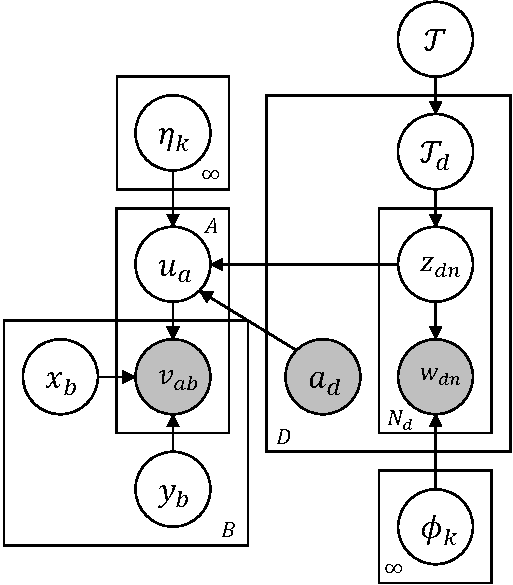
\includegraphics[width=\linewidth]{2015_teaparty/figs/snhdp}\\
%  \end{minipage}
%  \begin{minipage}[t]{0.32\textwidth}
%   \vspace{0pt}
%    \begin{small}
%    \begin{enumerate*}
%    	\item Generate a global tree $\mathcal{T}$: for each node $k$
%    	\begin{itemize}
%    		\item Draw topic $\phi_k \sim \mbox{Dir}(\beta)$
%    		\item Draw ideal point $\eta_k \sim \mathcal{N}(\mu, \sigma)$
%            \item Draw $\omega_k \sim \mbox{Beta}(\gamma^{\glob}, \pi)$
%            \item Draw $\theta_k \sim \mbox{GEM}(\alpha^{\glob})$
%    	\end{itemize}
%    	\item For each bill $b \in [1, B]$
%    	\begin{itemize}
%    		\item Draw $x_b \sim \mathcal{N}(0, \sigma_x)$
%    		\item Draw $y_b \sim \mathcal{N}(0, \sigma_y)$
%    	\end{itemize}
%    	\item For each word type $v \in [1,V]$, draw $\tau_v \sim \mathcal{N}(0, \sigma_v)$
%    \end{enumerate*}
%    \end{small}
%  \end{minipage}
%  \begin{minipage}[t]{0.43\textwidth}
%   \vspace{0pt}
%    \begin{small}
%    \begin{enumerate*}
%    	\item[4.] For each document $d$ authored by voter $a_d$
%    	\begin{itemize}
%    		\item Generate local tree $\mathcal{T}_d$: for each node $k$
%            \begin{itemize}
%              \item Draw $\omega \subtwo dk \sim \mbox{Beta}(\gamma^{\loc}, \omega_k)$
%              \item Draw $\theta \subtwo dk \sim \mbox{Dir}(\alpha^{\loc}, \theta_k)$
%            \end{itemize}
%    		\item For each token $n \in [1, N_d]$
%    		\begin{itemize}
%    			\item Draw a node $z \subtwo dn \sim \mathcal{T}_d$
%    			\item Draw word token $w \subtwo dn \sim \mbox{Mult}(\phi_{z \subtwo dn})$
%    		\end{itemize}
%    	\end{itemize}
%    	\item[5.] For each voter $a \in [1, A]$
%    	\begin{itemize}
%    		\item Draw ideal point \\$u_a \sim \mathcal{N}(\bar{\bm z}_a^T \eta + \bar{\bm w}_a^T \tau, \rho)$
%    		\item For each bill $b \in [1, B]$, the probability of $v \subtwo ab$ being
%    \textsf{Yes} is $f \subtwo ab = f(u_a x_b + y_b)$
%    	\end{itemize}
%    \end{enumerate*}
%    \end{small}
%  \end{minipage}
%\captionof{figure}{\small The graphical model and generative process of \name{} Ideal Point model. Hyperparameters
%are omitted for clarity.} \label{fig:snhdp}
%\end{minipage}
%\end{figure*}
%
%\paragraph{Generate global tree $\mathcal{T}$} The global tree $\mathcal{T}$ is generated using the nested Chinese
%restaurant process (nCRP). Proposed by~\cite{blei-07}, nCRP provides a flexible distribution over
%tree-like structures with unbounded width and depth. This is achieved by associating each node $k$
%in the tree with an infinite distribution over its children $\theta_k \sim
%\mbox{GEM}(\alpha^{\glob})$ and a biased coin $\omega_k \sim \mbox{Beta}(\gamma^{\glob},
%\pi)$.\footnote{In $\mbox{Beta}(\gamma^{\glob}, \pi)$, $\gamma^{\glob}$ is the scale and $\pi$ is
%the mean vector.} This construction was also used in earlier
%work~\cite{Adams:NIPS10,Nguyen:NIPSW13}.
%
%In addition, each node $k$ in the tree is also associated with a topic $\phi_k \sim
%\mbox{Dir}(\beta)$ and a regression parameter $\eta_k \sim \mathcal{N}(\mu,
%\sigma)$~\cite{nguyen-13:shlda}.
%
%\paragraph{Generate documents} Each document has its own distribution over nodes in the global tree,
%defined by the local tree $\mathcal{T}_d$~\cite{Ahmed:ICML13,Paisley:PAMI14}. [... Describe how
%$\mathcal{T}_d$ is generated.] [Describe nCRF by Ahmed et al. nHDP proposed is a similar model. The
%major difference is the termination process and the inference technique.]
%
%Each token $w \subtwo dn$ in our corpus is generated by first drawing a node $z \subtwo dn$ in the
%document-specific tree $\mathcal{T}_d$ and then drawing a word type from the corresponding topic
%$\phi_{z \subtwo dn}$. To draw a node from the local tree, we first start at the root and traverse
%downward. Assume the current node is $k$, we will stay at $k$ with probability $\omega \subtwo dk
%\sim \mbox{Beta}(\gamma^{\loc}, \omega_k)$. If deciding to move to a child node, we can move to an
%existing child or a new child.
%
%\paragraph{Generate vote outcomes} We model each voter's ideal point $u_a \sim \mathcal{N}(\bar{\bm z}_a^T \eta,
%\rho)$ where $\bar{\bm z}_a$ is a vector capturing how much attention that voter $a$ put on each
%topic in our hierarchy and is defined as $\bar{z} \subtwo ak = \frac{\sum_{d \in \mathcal{D}_a}
%\sum_{n=1}^{N \subtwo ad} \ind{z \subtwo dn = k}}{\sum_{d \in \mathcal{D}_a} N \subtwo ad}$
%where $\mathcal{D}_a$ denotes the set of documents authored by $a$ and $\ind{\mbox{\textsf{\small
%expr}}} = 1$ if $\small \textsf{expr}$ is true, and $0$ otherwise.
%
%\subsection{Inference}
%\label{sec:inference} We alternate among these steps
%\begin{itemize}
%  \item Sample a node for each token
%  \item Update the regression parameters
%  \item Update voters' and bills' ideal points
%\end{itemize}
%
%\paragraph{Sample node assignments}
%
%To assign a token $w \subtwo dn$ to a node in the tree, we first propose a node by sampling from an
%approximate conditional probability distribution over the tree nodes and then use the
%Metropolis-Hastings algorithm to either accept or reject the proposed node. Assume that token $n$
%of document $d$ is currently at node $k$ with level $l$ in $\mathcal{T}_d$, the probability that
%this token will stay at node $k$ is
%\begin{small}
%\begin{equation*}
%	\lambda^{\moveto kk} \subtwo dn = \frac{N \subtwo dk \minussuptwo dn}{N \subtwo d{\geq k} \minussuptwo dn + \gamma^{\loc}}
%	+ \frac{\gamma^{\loc}}{N \subtwo d{\geq k} \minussuptwo dn + \gamma^{\loc}}
%	\frac{N \subtwo {\cdot}k \minussuptwo dn + \gamma^{\glob} \pi_l}{N \subtwo {\cdot}{\geq k} \minussuptwo dn + \gamma^{\glob}}
%\end{equation*}
%\end{small}%
%where $N \subtwo dk$ is the number of tokens in document $d$ assigned to node $k$; $N \subtwo d{\geq k}$ is the number of document $d$'s tokens assigned to any nodes in the subtree rooted at $k$; $N \subtwo {\cdot}k$ is the number of tokens in all documents assigned to node $k$; and $N \subtwo {\cdot}{\geq k}$ is the number of tokens in all documents assigned to any nodes in the subtree rooted at $k$. We use the superscript $\minussuptwo dn$ to denote the exclusion of the assignment of token $n$ in document $d$ from the corresponding counts.
%
%If the token is not staying at $k$, it can move to either an existing child node $j$ of $k$ or a
%new child node $j^{new}$ of $k$. The probability that it will move to an existing child node $j$ is
%$\lambda^{\moveto kj} \subtwo dn = $
%\begin{small}
%%\begin{equation*}
%%	 (1 - \lambda^{\moveto kk} \subtwo dn)
%%	\left(\frac{N \subtwo d{\moveto kj} \minussuptwo dn}{N \subtwo d{\moveto k{\star}} \minussuptwo dn + \alpha^{\loc}}
%%	+ \frac{\alpha^{\loc}}{N \subtwo d{\moveto k{\star}} \minussuptwo dn + \alpha^{\loc}}
%%	\frac{N \minussuptwo dn \subtwo {\cdot}{\moveto kj}}{N \subtwo {\cdot}{\moveto k{\star}} \minussuptwo dn + \alpha^{\glob}}
%%	\right)
%%\end{equation*}
%\begin{equation*}
%	 (1 - \lambda^{\moveto kk} \subtwo dn)
%	\left(\frac{N \subtwo d{\moveto kj} \minussuptwo dn}{N \subtwo d{>k} \minussuptwo dn + \alpha^{\loc}}
%	+ \frac{\alpha^{\loc}}{N \subtwo d{>k} \minussuptwo dn + \alpha^{\loc}}
%	\frac{N \minussuptwo dn \subtwo {\cdot}{\moveto kj}}{N \subtwo {\cdot}{>k} \minussuptwo dn + \alpha^{\glob}}
%	\right)
%\end{equation*}
%\end{small}%
%where $N \subtwo d{\moveto kj}$ denotes the number of tokens in document $d$ moving from node $k$ to node $j$, $N \subtwo d{>k}$ denotes the number of tokens in document $d$ moving from node $k$ to any of its child node (i.e., $N \subtwo d{>k} = N \subtwo d{\geq k} - N \subtwo dn$).
%
%The probability that the token will move to a new child node $j^{new}$ is $\lambda^{\moveto k{j^{new}}} \subtwo dn = $
%\begin{small}
%\begin{equation*}
%	 (1 - \lambda^{\moveto kk} \subtwo dn)
%	\left(\frac{\alpha^{\loc}}{N \subtwo d{>k} \minussuptwo dn + \alpha^{\loc}}
%	\frac{\alpha^{\glob}}{N \subtwo {\cdot}{>k} \minussuptwo dn + \alpha^{\glob}}
%	\right)
%\end{equation*}
%\end{small}
%
%We propose a node by traversing from the root of the tree downwards, sample a node level-by-level.
%At each node $k$, we choose among the following three options with probabilities:
%%\begin{itemize}
%%  \item Stay on the current node $k$ with probability $\lambda^{\moveto kk} \subtwo dn \cdot
%%      \phi \subtwo k{w \subtwo dn}$
%%  \item Move to an existing child node $j$ with probability $\lambda^{\moveto kj} \subtwo dn
%%      \cdot \phi \subtwo j{w \subtwo dn}$
%%  \item Create a new child node $j^{new}$ of $k$ and move there with probability
%%      $\lambda^{\moveto k{j^{new}}} \subtwo dn \cdot \phi \subtwo {j^{new}}{w \subtwo dn}$.
%%      Since we put a symmetric Dirichlet prior over the topics, $\phi \subtwo {j^{new}}{w
%%      \subtwo dn} = 1/V$.
%%\end{itemize}
%
%$
%\left\{
%  \begin{array}{ll}
%    \lambda^{\moveto kk} \subtwo dn \cdot \phi \subtwo k{w \subtwo dn}, & \hbox{stay on $k$;} \\
%    \lambda^{\moveto kj} \subtwo dn \cdot \phi \subtwo j{w \subtwo dn}, & \hbox{move to existing child $j$;} \\
%    \lambda^{\moveto k{j^{new}}} \subtwo dn \cdot \phi \subtwo {j^{new}}{w \subtwo dn}, & \hbox{move to new child $j^{new}$.}
%  \end{array}
%\right. $
%The proposal probability for a node $k$ is $q(k) = $
%\begin{equation*}
%  \frac{\lambda^{\moveto kk} \subtwo dn \cdot \phi \subtwo k{w \subtwo dn}}
%  {\sum_{j' \in \mathcal{C}_k} \lambda^{\moveto k{j'}} \subtwo dn \cdot \phi \subtwo {j'}{w \subtwo dn}}
%  \prod_{(\moveto ij) \in \mathcal{P}({k})}
%  \frac{\lambda^{\moveto ij} \subtwo dn \cdot \phi \subtwo j{w \subtwo dn}}
%  {\sum_{j' \in \mathcal{C}_i} \lambda^{\moveto i{j'}} \subtwo dn \cdot \phi \subtwo {j'}{w \subtwo dn}}
%\end{equation*}
%The true probability of assigning $w \subtwo dn$ to node $k$ is \begin{equation*}
%	p(k) = \lambda^{\moveto kk} \subtwo dn
%	\cdot \phi \subtwo k{w \subtwo dn}
%	\prod_{(\moveto ij) \in \mathcal{P}({k})} \lambda^{\moveto ij} \subtwo dn
%\end{equation*}
%where $\mathcal{C}_i$ denotes the set of nodes which consists of $i$, all existing children of $i$
%and a new child of $i$ and $\mathcal{P}(k)$ denotes the path from the root to node
%$k$. Thus, assume the current node is $k^{\cur}$ and the proposed node is $k^{\prop}$, the according to the Metropolis-Hastings algorithm, we accept the proposed node with the probability of $\min \left(1,
%\frac{q(k^{\prop})}{q(k^{\cur})} \frac{p(k^{\cur})}{p(k^{\prop})}\right)$
%
%References~\cite{Kim:CIKM12}, \cite{Ahmed:ICML13}.
%
%\paragraph{Update topic regression parameters}
%\begin{equation*}
%	\mathcal{L}(\eta) = -\frac{1}{2\rho}\sum_{a=1}^A (u_a - \bar{\bm z}_a^T \eta)^2
%	- \frac{1}{2\sigma} \sum_{k \in \mathcal{T}} (\eta_k - \mu)^2
%\end{equation*}
%
%\paragraph{Update ideal point model's parameters}
%Update $u_a$, $x_b$ and $y_b$ using gradient descent. $\mathcal{L}(\bm u, \bm x, \bm y)$
%\begin{small}
%\begin{eqnarray}
%	&=& \sum_{a=1}^A \sum_{b=1}^B v \subtwo ab \log f \subtwo ab + (1 - v \subtwo ab) \log (1 - f \subtwo ab) \nonumber \\
%	&-& \sum_{a=1}^A \frac{(u_a - \bar{\bm z}_a^T \eta)^2 }{2\rho}
%	- \sum_{b=1}^B \frac{x_b^2}{2\sigma_x}
%	- \sum_{b=1}^B \frac{y_b^2}{2\sigma_y} \nonumber
%\end{eqnarray}
%\end{small}
%
%\paragraph{Improving identifiability using anchored voters}
%To avoid sign flipping, we initialize extreme voters with -3 and 3.
%
%\paragraph{Improving topic interpretability using priors}
%We use the major issues in Policy Agenda
%codebook~\footnote{\url{http://www.policyagendas.org/page/topic-codebook}} to label to first-level
%node in our hierarchy. The labeled data are from the Congressional Bill project
